\section{Introduction}\label{sec:introduction}

\subsection{An Observatory for Rare Events}

\begin{figure*}[!htbp]
\begin{center}
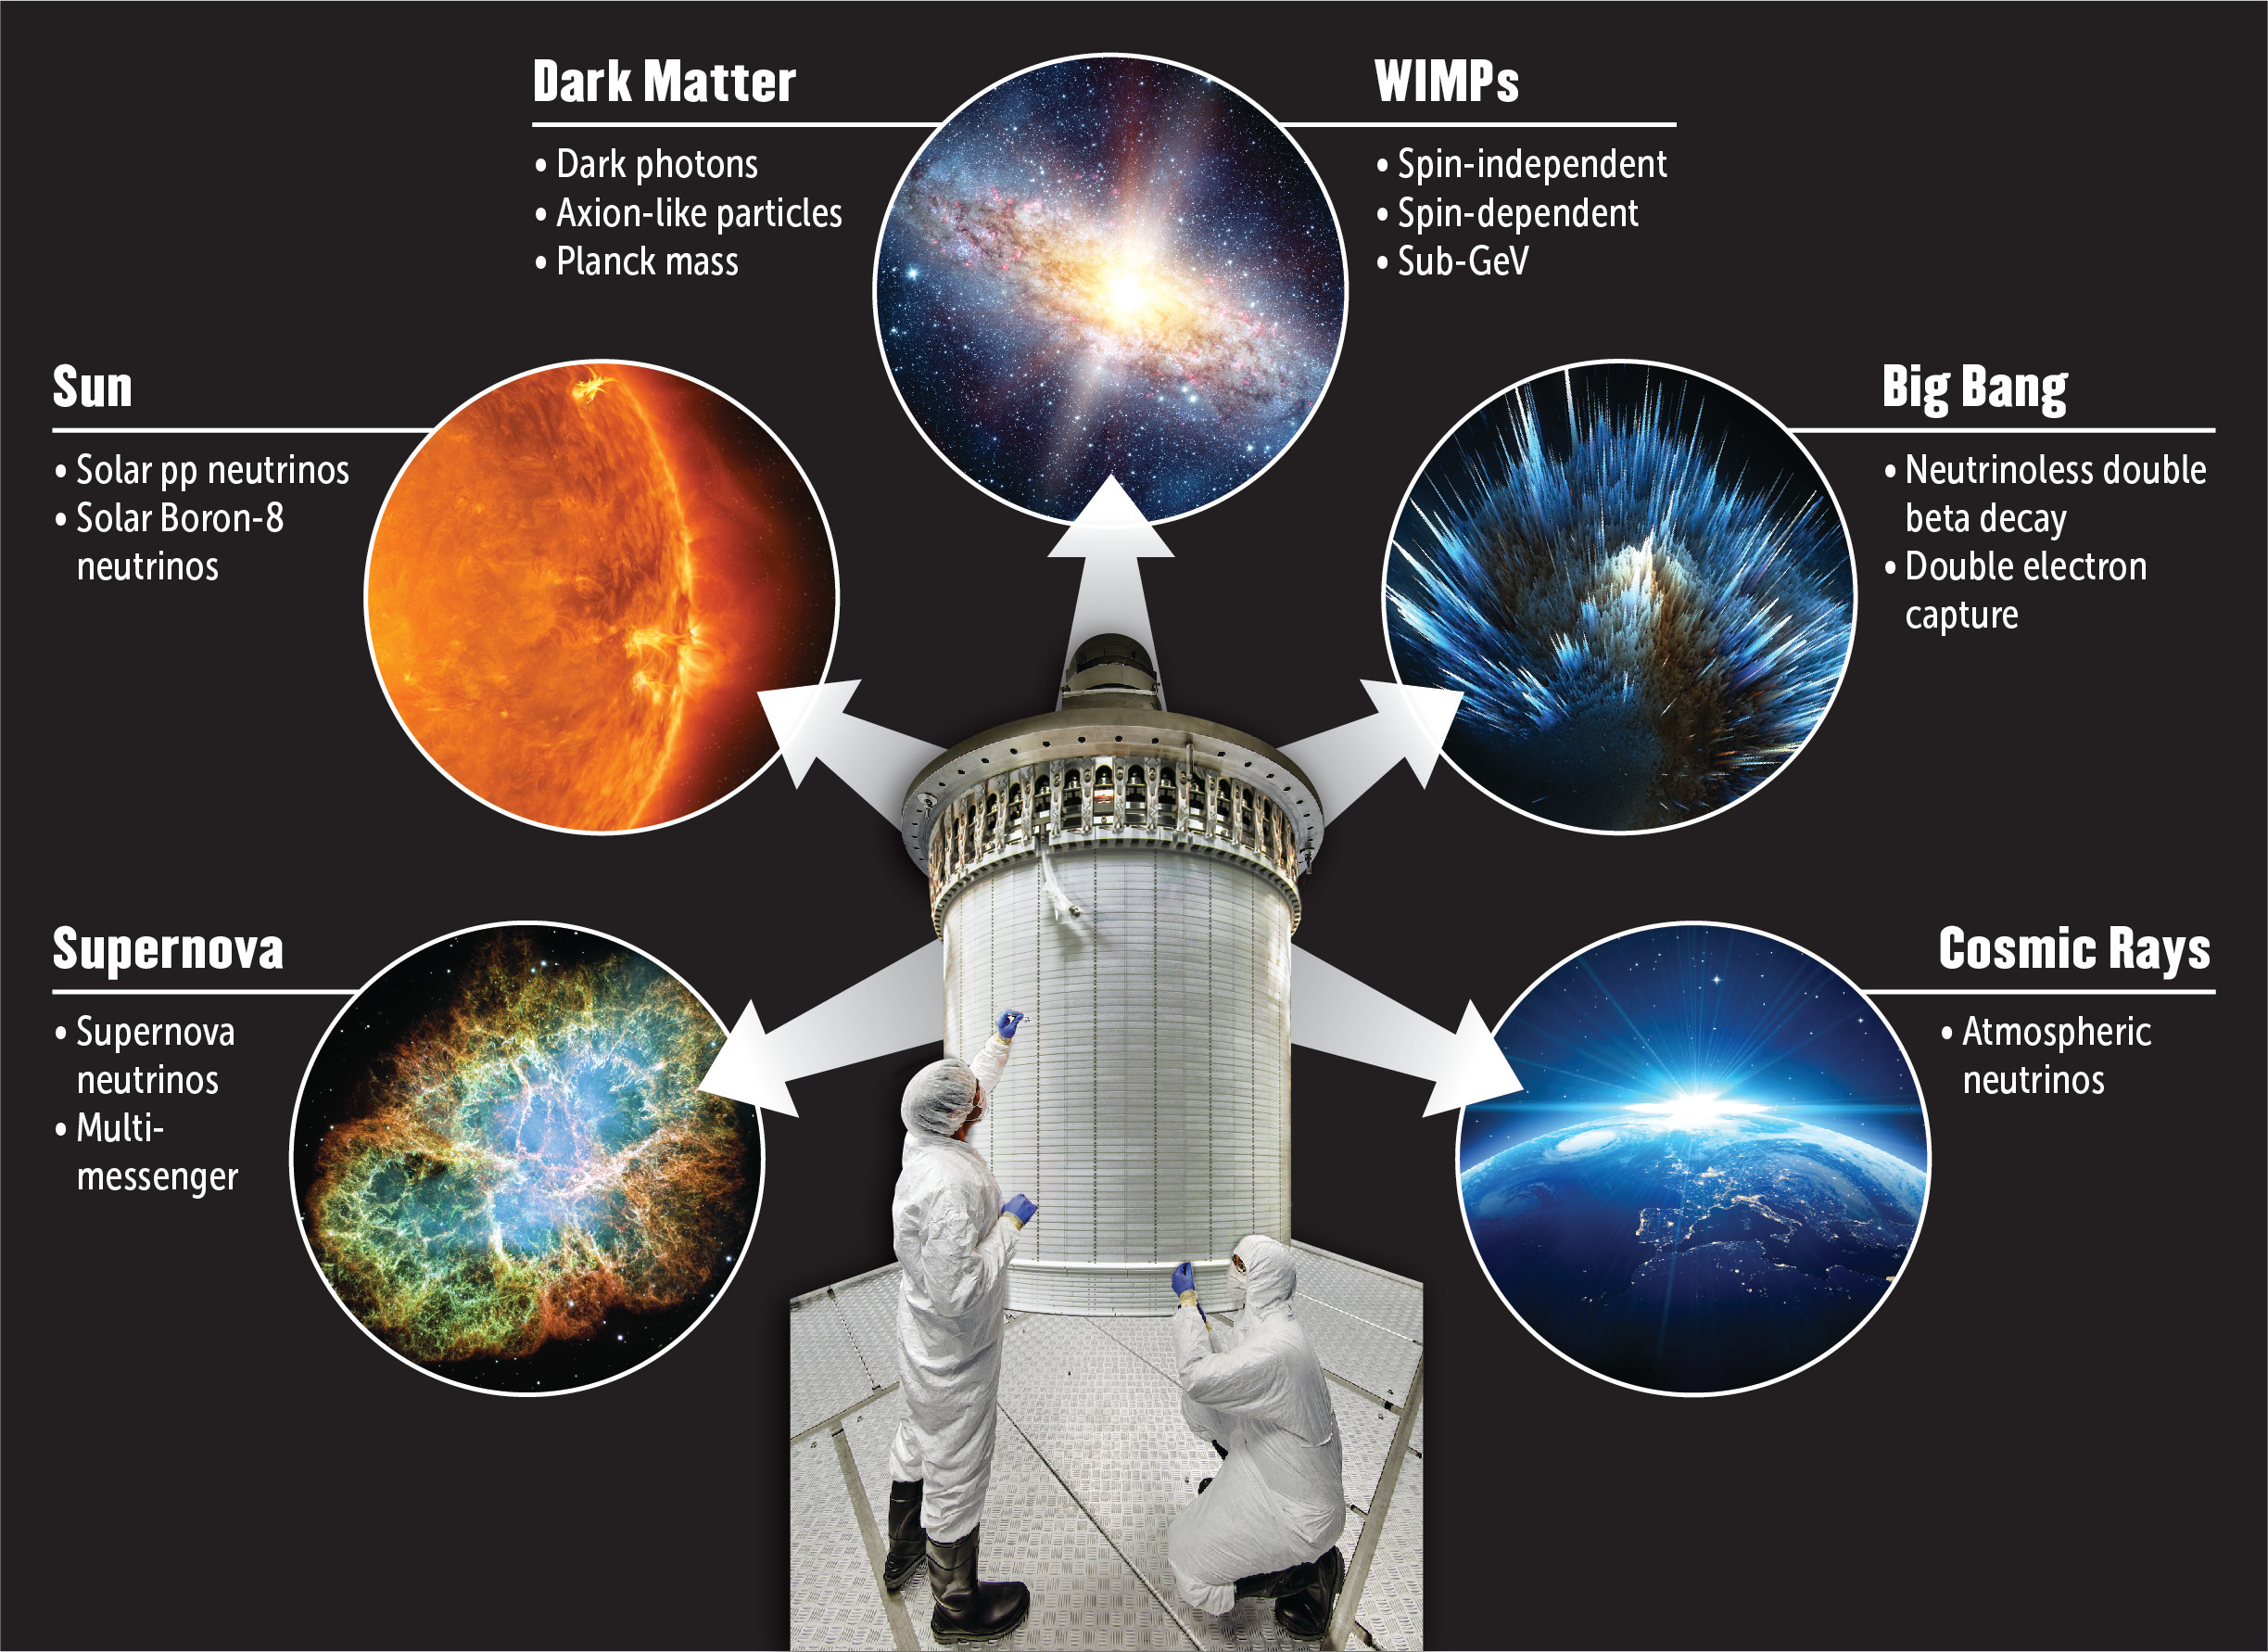
\includegraphics[width=2\columnwidth]{fig_sciencechannels.jpg}
\caption{The science channels of a next-generation liquid xenon observatory for rare events spans many areas and is of interest to particle physics and cosmology, nuclear physics, astrophysics, and solar physics.}\label{fig:sciencechannels}
\end{center}
\end{figure*}

Identifying the true nature of dark matter is one of the most important questions in physics today. As we show in this review, liquid xenon time projection chambers (TPCs) are the leading technology in searches for a large variety of dark matter particle candidates. Following two decades of evolution of this technology, now is the time to design the ultimate next-generation dark matter experiment in order to probe the widest possible range of dark matter candidates. A possible realization of such detector has been proposed by the DARWIN collaboration~\cite{Aalbers:2016jon}. As we show in this review, such an experiment also serves as a versatile astroparticle physics observatory that is sensitive to neutrinos from our Sun, the atmosphere, and Galactic supernovae. Further, this experiment will have competitive sensitivity to search for neutrinoless double-beta decay and other rare events. \autoref{fig:sciencechannels} illustrates these topics.

\subsection{Evidence for Dark Matter}

% history
Strong evidence on astronomical and cosmological scales suggests gravitational interaction between baryonic matter and an unknown type of non-luminous matter, called dark matter~\cite{Bertone:2004pz,Bertone:2016nfn}. In 1922, the Dutch astronomer Jacobus Kapteyn was among the first to use the word ``dark matter'' to refer to invisible matter whose existence is inferred only from its gravitational effects. At the time, it was thought that such dark matter consisted of obscure stars; these might have been extinct and dark or simply not bright enough to be seen. While Kapteyn found that the amount of dark matter in the Milky Way ``cannot be excessive''~\cite{Kapteyn:1922zz}, later that same year the British astronomer James Jeans came to another conclusion~\cite{Jeans:1922}. In fact, by reanalysing the data, Jeans realized that ``there must be about three dark stars in the universe to every bright star.'' The next decade, Jan Oort used the vertical kinematics of Milky Way stars to constrain the local dark matter content~\cite{Oort:1932}, while Fritz Zwicky became the first to use the virial theorem on galaxies to infer the presence of dark matter within the Coma Cluster~\cite{Zwicky:1933gu}. Further evidence for dark matter in galaxies came in 1978, when Vera Rubin an collaborators established that the rotation velocities of stars in spiral galaxies consistently differ from the distribution expected given the amount of baryonic matter~\cite{Rubin:1970zza}. 

% versatility of evidence
Since then, evidence for dark matter is found across all time and length scales~\cite{Lisanti:2016jxe}, spanning from the Big Bang to today, and from the cosmos as a whole down to individual galaxies~\cite{Kolb:1990vq}. Gravitational effects of dark matter can be observed in the cosmic microwave background, e.g.~with the Planck satellite~\cite{Akrami:2018vks}. Current estimates put the dark matter mass-energy density at five times that of baryonic matter in the observable universe~\cite{Aghanim:2018eyx}. Increased understanding of large-scale structure formation points to the existence of non-relativistic (cold) dark matter~\cite{Springel:2006vs,Knobel:2012wa,Coil:2012vw}. Gravitational lensing strongly suggests the presence of a significant amount of non-baryonic matter with no observable electromagnetic interaction~\cite{Bartelmann:1999yn}. 

% rotation curves
The critical role of dark matter in the formation of galaxies~\cite{Silk:2012ra} such as our own Milky Way~\cite{Read:2014qva} underlines its importance to humanity. Galactic rotation curves~\cite{Salucci:1996bf,Richards:2015gla} and dynamics~\cite{Sofue:2000jx,Foster:2010ri} provide evidence for the existence of a uniformly-distributed halo of dark matter around most galaxies. A precise determination of the local dark matter halo density is fundamental for interpreting results from direct detection experiments; however, density estimates are model-dependent and may vary depending on the method used~\cite{Read:2014qva,deSalas:2019rdi}. Methods used to determine the local dark matter density can be broadly classified into local methods and global methods. Local methods focus on a small volume around the solar system, while global methods analyse data over a much bigger volume and attempt to determine the local dark matter density based on our position within the halo. Based on global methods using Gaia data release~2~\cite{Brown:2018dum}, the local dark matter density has been determined to be in the range $\rho = (0.3-0.4)$~$\1{GeV/cm^3}$~\cite{deSalas:2019pee}, while local methods based on the same data have produced a wider range of $\rho = (0.4-1.5)$~$\1{GeV/cm^3}$~\cite{Hagen18,Buch:2018qdr,Widmark:2018ylf} with some tendency towards higher values~\cite{Wu:2019nhd}. When presenting results from direct dark matter searches, it is common to assume $\rho = 0.3$~$\1{GeV/cm^3}$~\cite{Baxter:2021pqo}, which results from mass modelling of the Milky Way using parameters in agreement with observational data~\cite{Green:2011bv}.

% need to search for it
While the existence of dark matter is thus well established, its physical characteristics remain elusive. Astrophysical observations indicate that dark matter could take the form of a new elementary particle outside the current Standard Model (SM) of particle physics~\cite{Tanabashi:2018oca}. The nature of this non-baryonic component is still unknown: its existence would be one of the strongest pieces of evidence that the current theory of fundamental particles and forces, summarized in the SM, is incomplete. A number of proposed candidates have been put forward over time, with some of the most popular candidates discussed in sections~\ref{sec:wimps} and~\ref{sec:broaderdarkmatter}.

\subsection{Dark Matter Direct Detection}

% history and basic idea
Since the 1980s, there have been large efforts to develop experiments on Earth that are able to directly search for dark matter, particularly for Weakly Interacting Massive Particles (WIMPs)~\cite{Drukier:1983gj,Smith:1983jj,Goodman:1984dc,Drukier:1986tm}, one popular dark matter candidate. Given the low expected interaction strength, the probability of multiple collisions within a detector is negligible, resulting in a recoil spectrum of single scattering events. A possible dark matter signature would be an annual modulation of the interaction count rate due to the motion of the Earth around the Sun~\cite{Goodman:1984dc,Drukier:1986tm}. The relative velocity of dark matter particles in the Milky Way halo with respect to the detector on Earth depends on the time of year; therefore, the measured count rate is expected to exhibit a sinusoidal dependence with time.

% a nod to other experiments
In the effort to directly detect dark matter, many technologies have been developed to measure dark matter interactions with target nuclei. Complementary searches with different targets, discussed further in \autoref{sec:complementarity}, are essential to tease out the nature of dark matter. In the most common approach, experiments attempt to measure the nuclear recoil energy produced by collisions between dark matter candidates and target nuclei in the detector. The recoiling nucleus can deposit energy in the form of ionization, heat, and/or light that is subsequently detected. Different technologies have been explored so far to achieve this goal~\cite{Schumann:2019eaa}. Successful targets include solid state crystals~\cite{Aalseth:2014eft,Agnese:2014aze,Armengaud:2016cvl,Shields:2015wka,Aguilar-Arevalo:2016ndq,CRESST:2019jnq,Crisler:2018gci} and dense noble liquids~\cite{Aalseth:2018gq,Akerib:2016vxi,Aprile:2017aty,Cui:2017nnn,Kobayashi:2018jky,Amole:2017dex}. 

\subsection{An Evolution of Scales}\label{sec:evolution}

\begin{figure}[!htbp]
\begin{center}
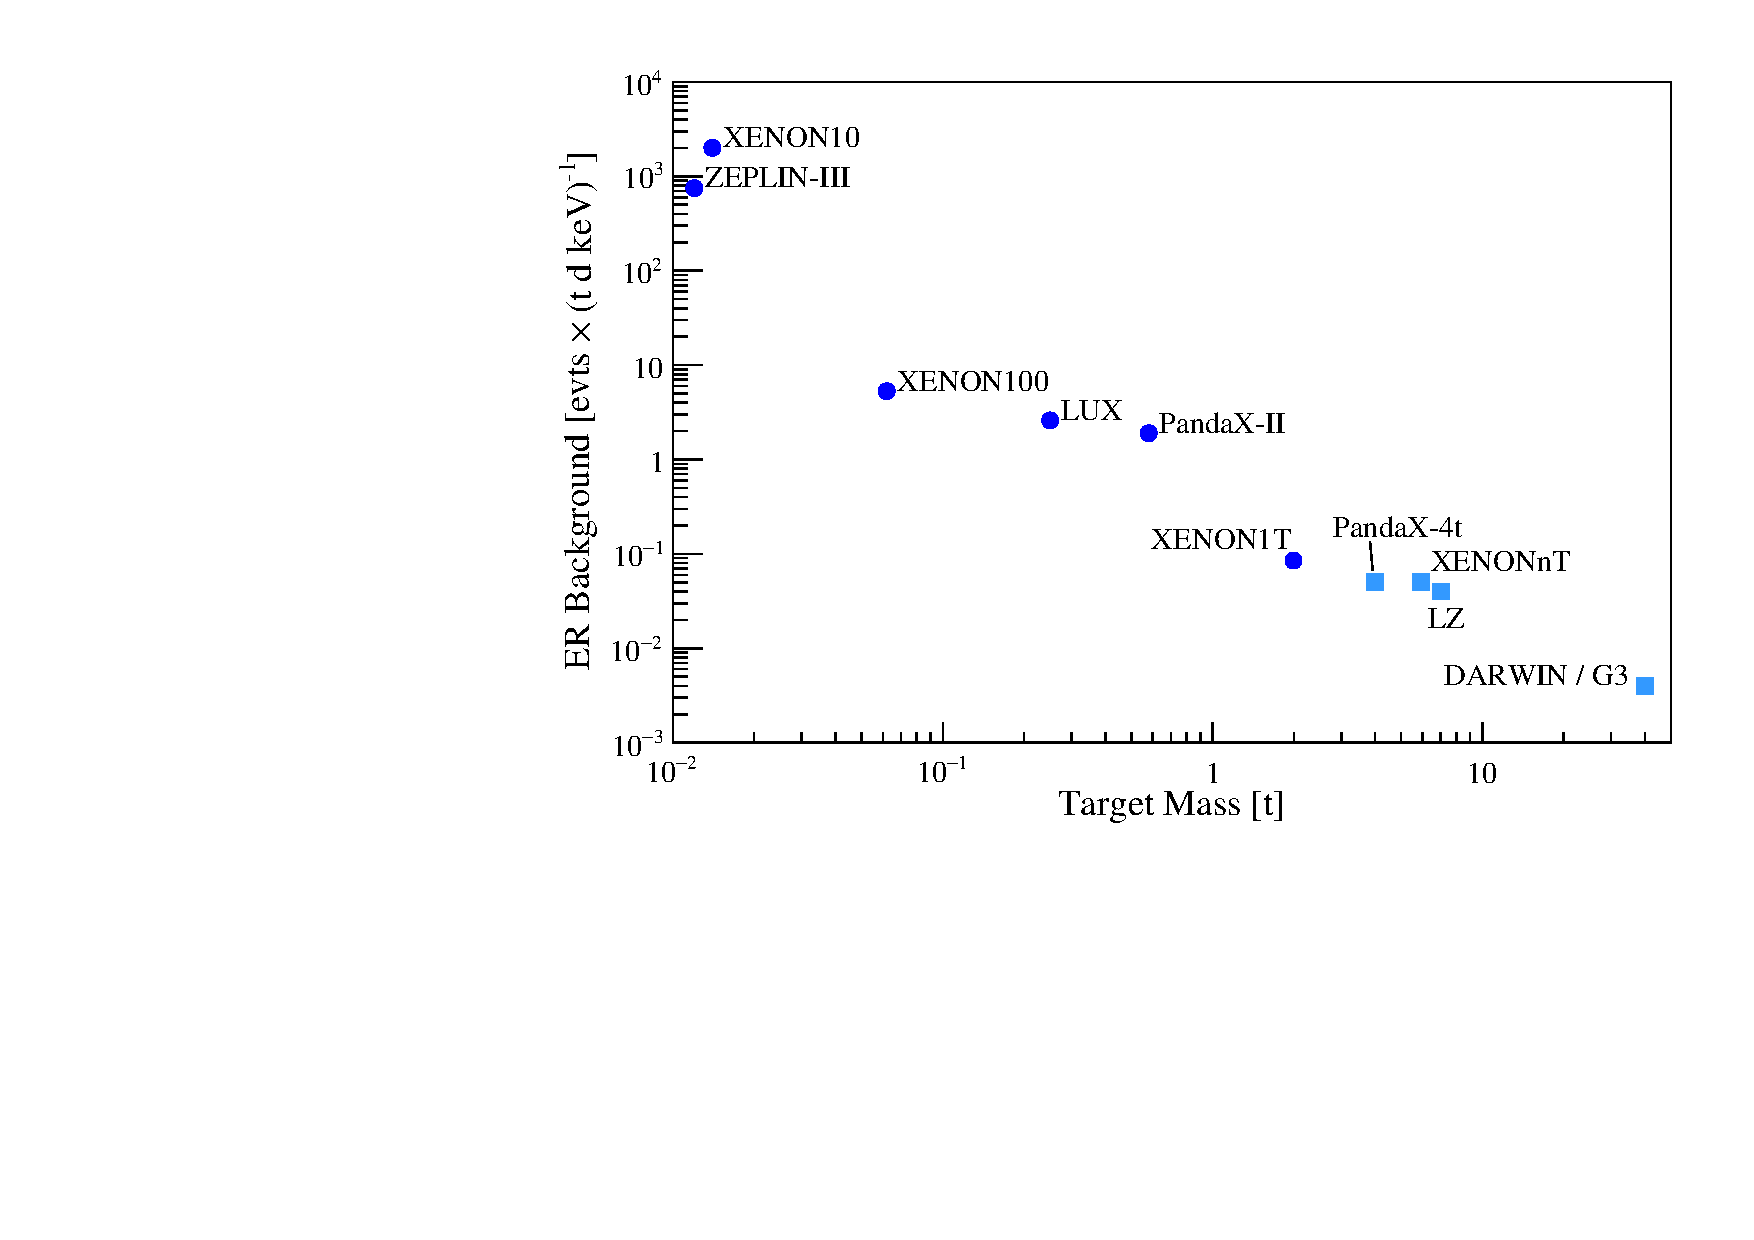
\includegraphics[width=0.9\columnwidth]{fig_evolution.pdf}
\caption{The backgrounds rates in liquid xenon TPCs (before discrimination) decreased exponentially over the years. Likewise, there has been an exponential gain in sensitivity. See text for references.}\label{fig:evolution}
\end{center}
\end{figure}

Liquid xenon TPCs in particular have demonstrated their exceptional capabilities for rare event detection as a result of an intense, decade-long development. The interested reader is referred to~\cite{Bolozdynya:2010, Akimov:2021} for detailed discussions of this technique. The two-phase (or dual-phase) emission detector that underlies liquid xenon TPCs was proposed a half-century ago~\cite{Dolgoshein:1970}. Its use for the detection of dark matter particles and neutrinos proposed in 1995~\cite{Bolozdynya:1995}, with more mature conceptional designs developed around the turn of the millennium~\cite{Cline:2000, Aprile:2002ef}. Evolving out of ZEPLIN-I~\cite{Alner:2005pa}, the ZEPLIN-II~\cite{Alner:2007ja} detector was the first two-phase xenon dark matter experiment, with both experiments setting competitive limits on WIMP interactions at that time. This technology was further advanced in ZEPLIN-III~\cite{Lebedenko:2008gb,Araujo:2011as} and with XENON10~\cite{Angle:2007uj} saw the first leading limits on WIMP interactions. XMASS in particular demonstrated the benefit of fiducialization in single phase detectors~\cite{XMASS:2018bid}. Further evolution progressed through successively larger, cleaner, and thus more sensitive detectors: from XENON100~\cite{Aprile:2011dd,Aprile:2012nq}, LUX~\cite{Akerib:2016vxi}, PandaX-I~\cite{Xiao:2014xyn} and PandaX-II~\cite{Wang:2020coa} to XENON1T~\cite{Aprile:2018dbl} and the current generation PandaX-4T~\cite{Zhang:2018xdp}, XENONnT~\cite{Aprile:2020vtw}, and LZ~\cite{Akerib:2018lyp} (\autoref{fig:evolution}). The next-generation experiment discussed here is labeled DARWIN/G3 in \autoref{fig:evolution} and as shown there~\cite{Schumann:2015cpa} represents a natural continuation of this evolution.

\subsection{The Liquid Xenon Time Projection Chamber}

\begin{figure}[!htbp]
\begin{center}
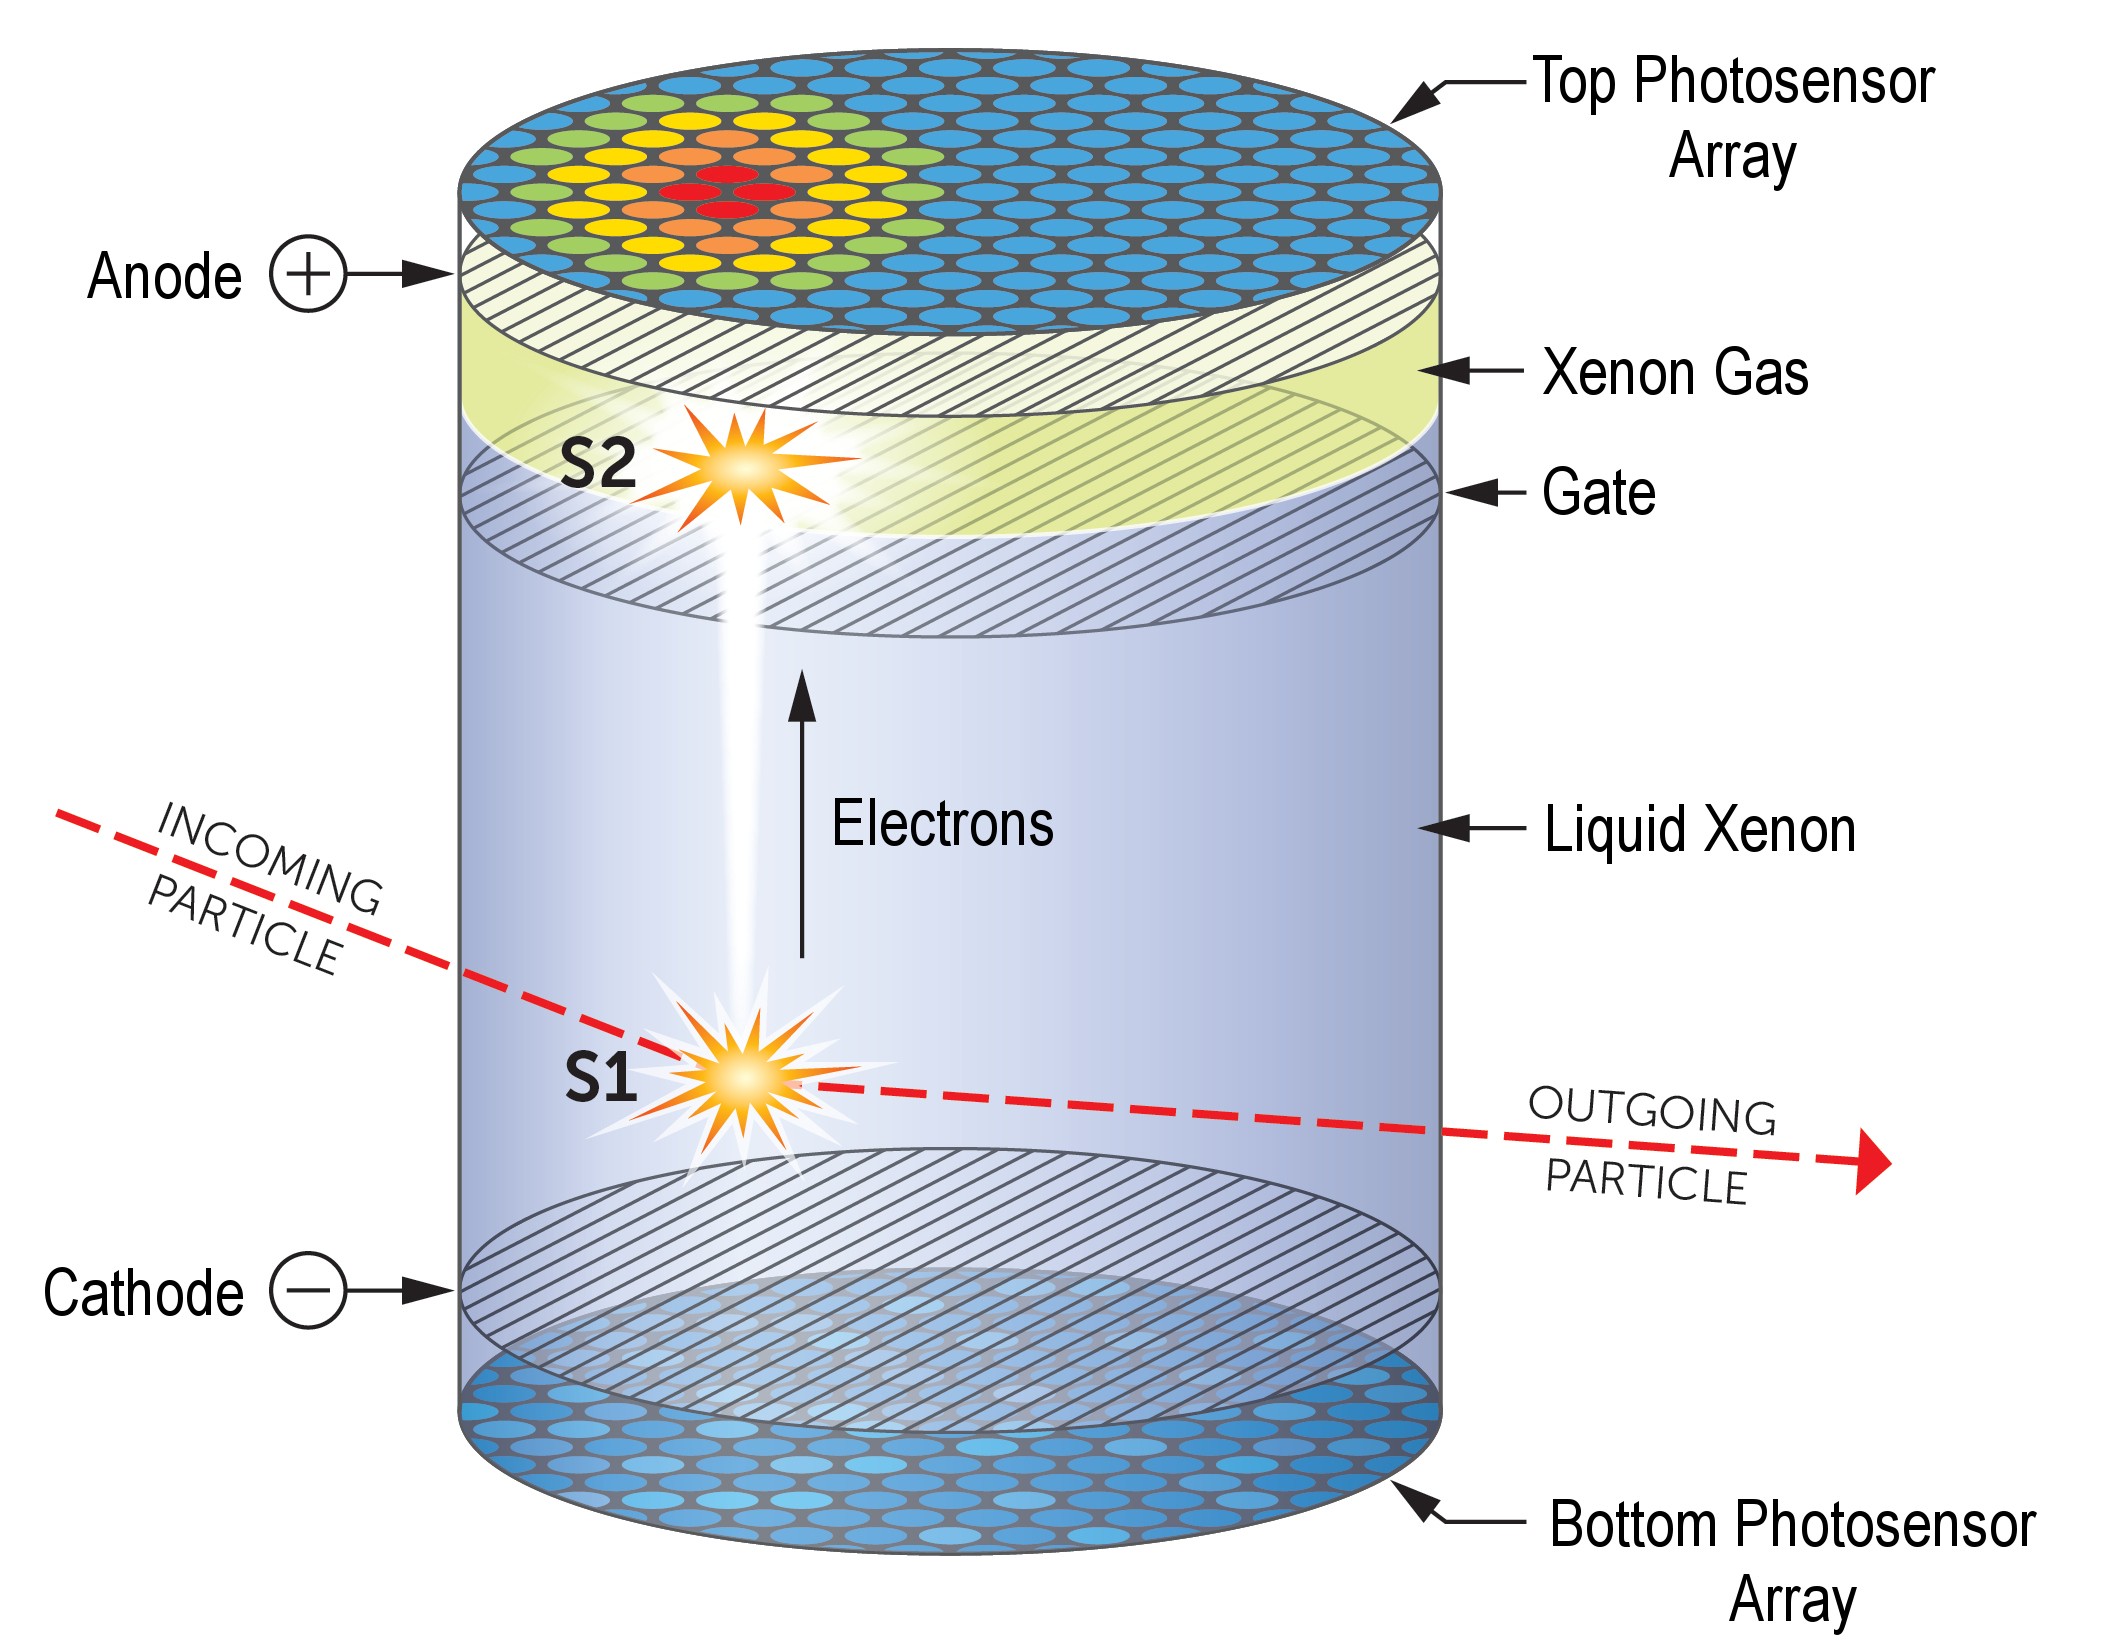
\includegraphics[width=0.99\columnwidth]{fig_tpc-mo_lifton.jpg}
\caption{Principle of a dual-phase liquid xenon time projection chamber. Energy from a particle interaction within the active liquid xenon volume produces prompt scintillation light (S1) and a delayed signal (S2) from electroluminescence (proportional scintillation) in the gaseous xenon layer. The localization of the S2 signal and the time difference between S1 and S2 allows for determination of the original vertex location.}\label{fig:tpcsketch}
\end{center}
\end{figure}

% basic layout 
A next-generation liquid xenon TPC will contain at least $\mathcal{O}(50)$ tonnes of liquid xenon as target for rare event searches. Conventionally, the liquid xenon volume will be surrounded by light reflectors for vacuum ultra-violet (VUV) light, allowing maximum light detection~\cite{Aprile:2004ey}. Two arrays of light sensors, such as photomultiplier tubes (PMTs)~\cite{Akerib:2012da,XENON:2015ara} or silicon photomultipliers (SiPMs)~\cite{Aprile:2005qq,Baudis:2020nwe}, are arranged on the top and bottom part of the TPC to detect light signals, see \autoref{fig:tpcsketch}. 

% minimal description to define the terms ER, NR, S1, S2, fiducialization. 
A particle incident on the liquid xenon target deposits energy and produces both prompt scintillation light and ionization electrons. The scintillation signal is immediately detected by the photosensors as the S1 signal. The \textit{active} liquid xenon volume is defined by a cathode and a gate electrode, separated by $\sim$3~meters to provide a drift field for the electrons. These drifting ionization electrons are then extracted into the gas phase above the liquid xenon, where, given a $\sim$5~kV/cm amplification field, they produce electroluminescent light (proportional scintillation)~\cite{Lansiart:1976}. This electroluminescence is then detected by the same photosensors and is known as the S2 signal~\cite{Yamashita:2003rc,Aprile:2004ey, Mount:2017qzi}.

The time delay between S1 and S2 in addition to the localization of the S2 light pattern on the top photosensor array allows precise reconstruction of the three-dimensional interaction vertex~\cite{Angle:2006rj}. Fiducialization in event selection enables an effective way to suppress external gamma background for all rare event searches and to minimize impact from effects near the imperfect TPC surface. The ratio of S2 and S1 signals further allows for discrimination between different types of interaction in the liquid xenon TPC: nuclear recoils (NR) and electronic recoils (ER). Nuclear recoils are most notably induced by neutrons, WIMPs, and through Coherent Elastic Neutrino-Nucleus Scattering (CEvNS), whereas electronic recoils are produced by external gamma rays and internal beta decays~\cite{Aprile:2005mz,Akerib:2020lkv}. Nuclear recoils exhibit a lower S2/S1 ratio and can therefore be distinguished from electronic recoils~\cite{Akerib:2020lkv}. Excellent energy resolution further helps to differentiate various signals from relevant background~\cite{XENON:2020iwh}. As we explain in \autoref{sec:s2only}, the scientific reach of these TPCs can be extended towards lower energies by dropping the requirement of the presence of an S1; this results in sensitivity to single electrons.

\subsection{Xenon as a Detector Medium}\label{sec:detector_medium}

Xenon as a detection medium exhibits several desirable features~\cite{Aprile:2008bga}, giving it a significant advantage as a target material. The low work function of 13.7\,eV, averaged over scintillation and ionization, leads to yields as high as $\sim$65 photons per keV for gamma rays $\mathcal{O}$(100~keV)~\cite{Lenardo:2014cva}, similar to other excellent scintillators such as NaI and CsI. For nuclear recoils, the yields are still $\mathcal{O}$(10\%) of that, even below $\sim$10~keV~\cite{Aprile:2018jvg,PandaX-II:2021jmq}. Energy resolutions better than 1\% have been achieved at MeV scales~\cite{XENON:2020iwh} and mm-level position resolution can be achieved even in large TPCs~\cite{Solovov:2011aa,Aprile:2012vw,Baudis:2020nwe}. 

Liquid xenon is a well-understood and well-characterized detector medium. Based on world data, its response can be accurately modeled using the Noble Element Simulation Technique (NEST), a code package to simulate interactions in liquid xenon (and argon) and their detection in a TPC~\cite{Szydagis:2011tk, Szydagis:2013sih, Lenardo:2014cva, szydagis_m_2020_3905382}. This includes various interactions of interest, such as electronic recoils induced by gamma and beta rays, nuclear recoils, energy deposits by alphas, and more complex decays such as that from $^{83\text{m}}$Kr. These models have been demonstrated to correctly reproduce the mean yields and their widths across a wide range of detector parameters and energies even down to $300\1{eV}$, making this simulation package a mature, comprehensive tool for liquid xenon experiments. As a result of this and other efforts~\cite{Sorensen:2008ec,Dahl:2009nta,Bezrukov:2010qa,Sorensen:2010hq,Mu:2013dga,Mu:2013pja,Wang:2016obw}, the light and charge yields are now well understood at a fundamental level, with good comparisons to extant calibration data sets, as a function of energy, ionization density $dE/dx$, drift electric field, extraction electric field, particle and interaction type, and in some cases even concerning density, phase, and angle of the recoil relative to the drift field. 

Liquid xenon may be naturally contaminated with radioactive isotopes that could produce a dark matter background, such as $^{85}$Kr or $^{222}$Rn. However, purification to very high levels has already been demonstrated in dark matter~\cite{Abe:2008py,Akerib:2016vxi,Aprile:2016swn,Aprile:2018dbl} and neutrinoless double-beta decay experiments~\cite{Albert:2014awa}. In particular for $^{85}$Kr, purity leves have been achieved that are already sufficient for the next-generation detector discussed here. Further advantages of xenon are obtained through its high charge number $Z$, mass number $A$, and density; these allow for self-shielding of gamma ray and neutron backgrounds, which will multiply-scatter, especially in the outer limits of the fiducial volume (\autoref{sec:backgrounds}). Xenon also contains odd-neutron isotopes for spin-dependent neutron coupling (\autoref{sec:sd}), and enough residual spin-dependent proton sensitivity to produce competitive results for that science channel. In addition, natural xenon possesses promising isotopes for the search for neutrinoless double-beta decay (\autoref{sec:0nubb}) and double electron capture (\autoref{sec:dec}). Finally, the mass of the xenon nucleus makes it kinematically ideal for WIMPs in the mass range above a few GeV/c$^2$.

% whitepaper overview
In the following sections, we highlight the science case for a large, next-generation liquid xenon TPC detector for astroparticle physics. In \autoref{sec:wimps}, we overview various WIMP dark matter models, and the expected sensitivity when probing such models. In \autoref{sec:broaderdarkmatter}, we discuss other dark matter models that a next-generation liquid xenon TPC is sensitive to. In \autoref{sec:doublebeta}, we review double-beta processes to probe physics beyond the Standard Model. In \autoref{sec:neutrinos}, we discuss the science channels using neutrinos for astroparticle physics and particle physics. In \autoref{sec:otherstuff}, we collect physics channels that are not part of the above categories. Mitigation and rejection of detector backgrounds is sketched out in \autoref{sec:backgrounds}. The relation of a next-generation liquid xenon TPC to other future experimental efforts is discussed in \autoref{sec:complementarity}. Finally, we review some of the already-documented support for such a detector in the particle physics community in \autoref{sec:priority} before concluding in \autoref{sec:summary}. 
